\chapter{Single-cell mRNA processing}
% This is only a test.
% \section{A section}
% Lorem ipsum dolor sit amet, consectetuer adipiscing elit. Nulla odio
% sem, bibendum ut, aliquam ac, facilisis id, tellus. Nam posuere pede
% sit amet ipsum. Etiam dolor. In sodales eros quis pede.  Quisque sed
% nulla et ligula vulputate lacinia. In venenatis, ligula id semper
% feugiat, ligula odio adipiscing libero, eget mollis nunc erat id orci.
% Nullam ante dolor, rutrum eget, vestibulum euismod, pulvinar at, nibh.
% In sapien. Quisque ut arcu. Suspendisse potenti. Cras consequat cursus
% nulla.

% \subsection{A Figure Example}
% \label{ssec:figure_example}

% This subsection shows a sample figure.

% \begin{figure}[h]
%   \centering
%   \includegraphics[width=0.5\textwidth]{sandiego}
%   \caption[Short figure caption (must be \protect{$< 4$} lines in the list of figures)]{
%   A picture of San Diego.  Note that figures must be on their own line (no neighboring text) and captions must be single-spaced and appear \protect\textit{below} the figure.  Captions can be as long as you want, but if they are longer than 4 lines in the list of figures, you must provide a short figure caption.\index{SanDiego}}
%   \label{fig:sandiego}
% \end{figure}

% \subsection{A Table Example}

% While in Section \Cref{ssec:figure_example} Figure \Cref{fig:sandiego} we had a majestic figure, here we provide a crazy table example.


% %%%% TABLE 1 %%%%
% \vspace{0.25in}
% \begin{table}[!ht]
% \caption[Short figure caption (must be \protect{$< 4$} lines in the list of tables)]{A table of when I get hungry.  Note that tables must be on their own line (no neighboring text) and captions must be single-spaced and appear \protect\textit{above} the table.  Captions can be as long as you want, but if they are longer than 4 lines in the list of figures, you must provide a short figure caption.}

% \vspace{-0.25in}
% \begin{center}
% \begin{tabular}{|p{1in}|p{2in}|p{3in}|}

% \hline
% Time of day & Hunger Level & Preferred Food \\

% \hline
% 8am & high & IHOP (French Toast) \\

% \hline
% noon & medium & Croutons (Tomato Basil Soup \& Granny Smith Chicken Salad) \\

% \hline
% 5pm & high & Bombay Coast (Saag Paneer) or Hi Thai (Pad See Ew) \\

% \hline
% 8pm & medium & Yogurt World (froyo!) \\

% \hline
% \end{tabular}
% \end{center}
% \label{tab:analysis3}
% \end{table}

\section{Introduction}
The human body contains an estimated $3.72\times 10^{13}$ cells  \cite{Bianconi2013-jr}, all of which are highly specialized in form and function, and yet despite their incredible diversity in phenotypes, each cell contains nearly identical genotypes. These cells are heterogeneous because of their different RNA, protein, and metabolite molecules, which coordinately regulate the cell to express precise phenotypes. To study the variation between cells, we turn to single-cell analysis.

The original tool for single-cell analysis is the microscope  \cite{Hooke1665-bk,Van_Leeuwenhoek_undated-gu}, which can visualize structural differences between individual cells, but the molecules that create these differences are too small to resolve in live cells by current microscope technology. To compare the molecules of single cells, recent advances in microfluidics have allowed for capture of one cell at a time, which can be coupled with modern high-throughput technology to measure many messenger RNA (mRNA) molecules per cell, and together these are combined to create single-cell RNA-sequencing (scRNA-Seq)  \cite{Kolodziejczyk2015-wj,Ziegenhain2016-gb}. Computational analysis of these high-dimensional data can identify distinct cellular states or delineate cellular trajectories (reviewed by  \citet{Bacher2016-ze,Cannoodt2016-mt,Liu2016-cw,Trapnell2015-vn,Stegle2015-tl}).

While single-cell capture has enabled probing of cellular state measured through mRNA abundances, the study of an mRNA molecule's rich life (\Cref{fig:singlecell_questions}a) from birth (transcription) to death (degradation), the collection of actions known as mRNA processing  \cite{Blanc2003-wk,Gerstberger2014-hj,Yeo2016-do,Nussbacher2015-kr,Singh2015-gd}, has only started to be addressed at the single-cell level. As in bulk RNA-seq  \cite{Anders2012-fq,Kleinman2012-td,Lianoglou2013-pc,Nishikura2010-dk,Park2012-av,Peng2012-ru,Shen2014-zq,Wang2008-xh}, scRNA-seq has enabled the investigation of RNA processing features that are measureable by sequencing, such as alternative splicing, RNA editing, and alternative polyadenylation  \cite{Karlsson2017-wy,Marinov2014-iw,Picardi2017-bv,Shalek2013-ez,Velten2015-zd,Welch2016-it}. However, the high-throughput nature of scRNA-seq captures only the abundance of RNA transcripts in a snapshot in time and loses the information of RNA modifications, dynamics, localization, binding partners, and secondary structure. Thus, these features must be measured a different way.

Ideally, we would capture the entire cellular and molecular context of an RNA molecule. To accomplish this, we turn back to the microscope, a tried and true tool. While even the highest resolution microscopes cannot discern individual molecules without significant amplification  \cite{Femino1998-ws,Raj2009-ni}, microscopy captures cellular context including morphology and subcellular localization, and in the case of live-cell imaging, dynamics. Microscopy is limited by the ability to design fluorescent constructs to visualize RNA and protein molecules, and as a result, can only be performed for a few targets a time. Middle-ground technologies that are relatively high-throughput but also measure several aspects of the same cell or same transcript  \cite{Gierahn2017-ko,Macaulay2017-tb} have highest potential for discovery.
We will review the available methods to probe RNA processing at the single cell level, and highlight the current limitations, showing opportunities for novel technology to make breakthroughs in the knowledge of RNA processing.

% --- BEGIN manual facingcaption --- %
\clearpage
\thispagestyle{facingcaption}
\begin{figure}[h]
\captionsetup{labelformat=prev-page}
\caption[Overview of open questions in single-cell RNA processing.]{\textbf{Overview of open questions in single-cell RNA processing.}\\
\textbf{a.}~Overview of the processing steps in an RNA's life cycle: transcription (biogenesis), alternative splicing, poly-adenylation, modification, export, localization, translation, and degradation.\\
\textbf{b.}~Dichotomy of investigating distribution of transcripts across cells with high-throughput methods, and distribution of transcripts within cells using high-resolution methods.\\
\textbf{c.}~Examples of high-throughput measurements, where many transcripts can be measured at once, but only one feature of them may be measured.\\
\textbf{d.}~Examples of high-resolution measurements, where only a few transcripts can be measured at once, but many features of them can be profiled.
}
\label{fig:singlecell_questions}
\end{figure}
\clearpage
\begin{figure}[h]
\ContinuedFloat
\captionsetup{labelformat=empty}
\centering
% \includegraphics[width=5.8in]{sandiego.jpg}
\includegraphics[width=5.8in]{figures/singlecell_questions.pdf}
\end{figure}
%and, I'm not sure why, but one of the times I used this code the figure number wasn't augmented for the next figure, so check your figure numbers and if necessary uncomment the following line
%\addtocounter{figure}{1}
\clearpage
% --- END manual facingcaption --- %


\section{Balancing high-throughput and high-resolution single-cell technologies}

A complex tissue such as the human brain contains many different transcripts, but by measuring them at the bulk level, the cell of origin for each transcript is unknown (\Cref{fig:singlecell_questions}b, left). Using single-cell technologies, we quantify an RNA processing event either as presence or absence (e.g. m6A or splicing) or a continuous quantity (e.g. abundance or poly-A tail length). With these quantifications in hand, we want to be able to capture individual cells and measure each cell's transcripts to understand two separate questions (\Cref{fig:singlecell_questions}): How are transcripts distributed (1) across cells, and (2) within cells?

The questions of distributions of transcripts across cells and within cells represent the ends of a spectrum, each with their own advantages and limitations. Where on the one extreme there are high-throughput methods which can measure many transcripts per cell, but are low-resolution and can only measure one aspect, abundance, and on the other extreme are high-resolution methods which can measure a limited number of transcripts (low-throughput) but can measure many aspects beyond abundance, such as dynamics and localization.

To measure RNA processing across cells, we use high-throughput single-cell technologies to study cellular biology and answer the question, is a particular RNA processing event found only within certain subpopulations of cells, or does it co-occur within individual cells? If it's found within the same cell, are these on the same transcript, or on different transcripts in individual cells? Since these technologies only extract a snapshot in cellular time, akin to a still frame in a movie, we don't know how these transcripts change over time or how they are physically used within an individual cell, and thus high-throughput technologies are hypothesis-generating experiments. 

To test these hypotheses, we turn to low-throughput, high resolution technologies in molecular biology, which can answer the question, within cells, are the different transcripts differentially localized in different populations? Does the transcript have different temporal dynamics? Does it have different interactors, binding partners, or three-dimensional structure? To truly understand this, we would need to follow up with an experiment that turns the process of or over expresses it to see how it affects cellular fate.

\subsection{High-throughput}
We define ``throughput'' as the number of different molecules that can be measured at once from a single cell (\Cref{fig:singlecell_questions}c). High-throughput methods such as scRNA-Seq can measure ~18,000 transcripts per cell (~2000 genes/cell) for up to one million cells  \cite{noauthor_undated-xt}. These high-dimensional datasets can be used to study two main questions regarding the distribution of transcripts across cells  (\Cref{fig:singlecell_questions}b): (1) Do these processes co-occur on the same transcript, or on different transcripts within the same cell? (2) If they occur in different cells, do these cells comprise distinct population sub-structures? Digging into the population sub-structures can especially elucidate novel cell states or types, and understanding of cellular biology. Thus, high-throughput methods allow for measurement of one feature across many targets, and are especially enable the deep study of cellular biology and cell state.

High-throughput technologies come at the cost of resolution: many scRNA-seq techniques measures only the abundance of the 5' end of the mature, poly-adenylated mRNA  \cite{Kolodziejczyk2015-wj,Macosko2015-rl,Ziegenhain2016-gb}, thus missing large portions of the transcripts, the immature pre-mRNA and due to sequencing technology limitations, these methods cannot measure nucleotide modifications. Additionally, these measurements are destructive and the original cells cannot be restored to re-analyze to observe how they would respond to perturbations. If we develop a hypothesis from the high throughput data, we must test it on completely new and independent cells. Thus, high-throughput data such as scRNA-seq represents only a snapshot in time and loses the dynamics of the transcript's biogenesis, the localization of the transcript in the cell, its interactors, and any modifications or secondary structure.

The digital measurements of high-throughput data are necessarily lossy in part because the technology itself defines what can be observed, and all other features remain undetected. This echoes Jaron Lanier's ``You are Not a Gadget''  \cite{Jaron2010-hk} which discusses how the digital representation of an object inevitably removes all unmeasured features, and this can be problematic as they are still a part of the object. As an analogy, digitizing an impressionist painting as a photo does not capture the time of day the flax seeds were pressed to create the oil paints, the tautness of the muslin cloth on the frame, or the names of every person who has ever viewed the painting, but all of these are part of the history of the painting. These are examples of incidental measurements that are lost as soon as the object is digitized, because by digitizing, you've made decisions about what you think is important, and lose information about what you've chosen not to measure. Thus, as soon as you measure the abundance of a cell's transcripts through RNA-seq, you lose all other features of the transcript, such as its structure and nucleotide modifications, its localization and binding partners, its lifespan, and even more unmentioned features which have not yet been observed but could contribute to the RNA molecule's biography.


Finally, high dimensional data requires many computational manipulations  \cite{Bacher2016-ze,Cannoodt2016-mt,Stegle2015-tl}, which could retreat from the biology. Due to the lossy nature of the digital measurements, computational methods may not retain the biology as the algorithm may latch onto signals that are artefacts of the technology, rather than true biology. To many, the enormous amounts of data may feel like staring into ``tea leaves'' and trying to draw conclusions, and rigorous follow up and investigation across multiple algorithms is required to ensure the analysis is biologically correct. Thus, while high-throughput single-cell measurements such as RNA-Seq allow for exploration of huge biological datasets and digging into cellular populations, they are limited in their ability to study multiple features of an mRNA transcript's life cycle at once.

\subsection{Low-throughput}

To become closer to the biology, we turn to lower-throughput techniques such as microscopy, which allows for observation of dynamics and localization, trends that are not currently visible in high-throughput data (\Cref{fig:singlecell_questions}d). While almost an antediluvian tool, microscopy, especially fluorescence and confocal microscopy heavily used in single-cell analyses, has undergone many advances in resolution and throughput, allowing for visualization of RNA and protein molecules in thick (millimeter) tissue slices \cite{Buxbaum2015-eu,Shah2016-ut,Treweek2015-ri,Yang2014-xq}. To further investigate the subcellular characteristics such as time scales and localization, of RNA processing, we turn to low throughput analyses to answer two main questions: (1) Do the processes exist at the same or different, time and place? (2) What is the fate of transcripts with different RNA processing features? For example, if a gene's transcript with distinct RNA features co-occur in the same cell, how does the cell use the diverse transcripts differently? By studying RNA processing in both time and space, we will become ever closer to a deep understanding of the regulation of RNA.

\subsection{``Goldilocks'' balance of throughput and resolution}

Technologies that balance both throughput and resolution that are ``just right,'' as in the children's fairy tale of where the Goldilocks character finds the perfect porridge that isn't too salty or too sweet. These in-between methods are currently limited in the still-growing field of technological development in single cells and are a major need. Most technological innovation has focused on increasing either throughput or resolution, but we argue that the large leaps will be made by combining the two to show several aspects of a single RNA transcript molecule, in a way that has never been seen before. For example, in situ sequencing
 \cite{Chen2015-pv,Crosetto2015-hf,Ke2013-iu,Lee2015-fj,Lubeck2014-re,Shah2016-ut,Shah2016-sn} combines localization of transcripts with high-throughput microscopy or sequencing to spatially resolve transcripts within, and across cells. Other combination technologies include single-cell multiomics methods which measure several aspects of a cell at once, to answer the questions of how DNA mosaicism or epigenetics contribute to gene expression  \cite{Angermueller2016-rx,Hou2016-zi,Macaulay2017-tb,Reuter2016-op}, or how RNA levels influence protein levels with Seq-well. The development of methods which maximize the ``bang for the buck'' -- i.e. high-throughput while retaining cellular context -- will revolutionize single-cell biology and create opportunities for novel biological questions.

\section{Insights into RNA processing through single-cell technologies}

Here we discuss the aspects of RNA processing that are measurable by current technologies, and summarized in \Cref{fig:singlecell_central_dogma_methods}.

\begin{figure}[h]
  \centering
  \includegraphics[width=5.8in]{figures/singlecell_central_dogma_methods}
  \caption{Overview of what can be measured at different steps of the central dogma in terms of RNA processing.}
\label{fig:singlecell_central_dogma_methods}
\end{figure}

\subsection{Chaotic, ``bursty'' transcription is harmonized by slow nuclear export}

Single-cell analyses have long showed that cells do not constantly transcribe genes, but rather do it in a, stochastic ``bursty'' fashion  \cite{Kaern2005-ca,Kaufmann2007-nh,Raj2008-er,Raj2006-vi}. Single-molecule imaging paved the way to show the stochasticity of gene expression within genetically homogeneous cell populations \cite{Raj2006-vi,Vargas2011-iq} (, and was confirmed by single-cell RNA-Seq, which also showed bursty and cyclical transcriptional kinetics that would otherwise be masked in bulk sequencing data  \cite{Buettner2015-mj,Livak2013-nv,Shalek2013-ez}. How does the cell deal with what appears to be such chaotic creation of RNA? Two papers showed that while sudden bursts of expression in the nucleus are common, mRNAs aren't immediately exported to the cytoplasm  \cite{Bahar_Halpern2015-dq,Battich2015-df}, suggesting the mRNAs are first sequestered in storage facility before they are exported. Thus, bursty transcription is tempered with a slow drip of RNA export from the nucleus.


\subsection{Variability in isoforms is nonrandom but functional implications remain unclear}

Alternative splicing (AS) is a co- and post-transcriptional modification of mRNA that is a mechanism for proteomic diversity  \cite{Ameur2011-wf,Black2003-fz,Caceres2002-el,Day2016-ej,Kornblihtt2013-gm,Lee2015-vi}. AS removes introns, sequences from the immature mRNA which are not contained in the mature, poly-adenylated mRNA. Since the outcome of AS is the presence or absence of an intron, this can be readily measured using RNA-sequencing (RNA-Seq)  \cite{Wang2008-xh}. RNA-seq is a readily available technology for single cells and thus AS analysis can be directly applied. We discuss below the applications of single-cell analyses to studying alternative splicing.

Overall variation of AS in single cells can be studied using high-throughput methods such as RNA-sequencing. While bulk measurements show that individual isoforms may vary within a population, this doesn't show how individual cells use different transcripts. Understanding how individual cells choose one transcript or another has been challenging to measure. Do cells tend to have only one isoform of a gene, or do they contain many? One question that RNA-seq AS analysis can answer is, unbiasedly, which splicing events are changing within a cell population, or across cell populations? One early study found variability in isoforms using RNA fluorescence in situ hybridization (FISH) \cite{Waks2011-ye}. The earliest scRNA-seq study found that single-cell AS was more ``all or nothing'' -- each cell tended to have only one isoform, compared to bulk samples, which showed many isoforms \cite{Shalek2013-ez}. This shows that individual cells tend to only have a single isoform, and that variation in isoform composition, such as having multiple isoforms, is likely observed in bulk samples because of the heterogeneity of cells, rather than heterogeneity of transcripts within cells. Completeness of splicing is also associated with higher conservation of introns and exons \cite{Faigenbloom2015-jo}. Another study used full-transcript scRNA-seq to find that single cells had higher percentages of novel splice junctions than bulk data \cite{Marinov2014-iw}. Another study looked at alternative splicing in single cells captured from the mouse visual cortex and found changes in alternative splicing throughout the different cortical layers \cite{Tasic2016-et}. Another study developed statistical models to find variable splicing events across single cells, and applied this to find splicing events that change with cell cycle \cite{Welch2016-it}. Contrary to the initial study that most splicing events are ``all or nothing,'' another study used UMIs coupled with long-read sequencing to extract poly-adenylated mRNAs from from mouse oligodendrocytes and vascular and leptomeningeal cells \cite{Karlsson2017-wy}. They found a purifying selection of exon splice sites in protein coding genes, with very few junctions mapping to mis-spliced exons. They found up to 25 isoforms per cell, with most isoform differences occurring due to alternative transcription start and end sites, rather than cassette exons or 3' or 5' end positional differences. Earlier studies also showed that the choice of 3' isoform is highly variable, more variable than random selection \cite{Velten2015-zd}, a finding that was confirmed by RNA-FISH. More work is needed to analyze the choice of final exons, which can be aided by advances in computational methods for end-sequence analysis \cite{Derr2016-pj}. These results show that overall, alternative transcript architectures are highly variable in a statistically significant manner, but the purpose of this variation is still unknown. The ability to decipher whether there is function in the variability \cite{Arbel-Goren2014-iq,Dueck2016-mr,Symmons2016-xn,Yap:2016iga} is limited by the capture methods of transcripts, and is limited to highly-expressed transcripts.

The dynamics of splicing can be studied using microscopy of fluorescently labeled transcripts. For example, the competition between transcript release and splicing of the final intron of human beta-globin was found to favor transcript release, then splicing. Interestingly, splicing of diffuse RNA occurred rapidly, faster than diffusion \cite{Coulon2014-he} and alternative splicing is known to occur primarily after transcription \cite{Vargas2011-iq}. These studies have shed light onto how the transcription of RNA is decoupled from the creation of alternative transcripts.

The differential usage of the same gene's isoforms remains an interesting question. Why would a cell contain multiple isoforms? What are their different functions \cite{Yap:2016iga}? For example, the cell polarity gene Cdc42 has two possible terminal exons, exon 6 and exon 7, but in non-neuronal cells, exon 6 is strongly suppressed by polypyrimidine tract binding protein (PTB/Ptbp1) and only exon 7 is included \cite{Yap2016-dl}. However, in neurons, Ptbp1 is not expressed, and both exon 6 and exon 7 transcripts are expressed in equimolar ratios, disrupting this equimolar concentration resulted in defects in neuronal development. Too much of the exon 6 isoform led to insufficient axonogenesis and too much of the exon 7 isoform led to insufficient dendritic maturation. This suggests the exact ratios and distributions are critical for normal neuronal development.


\subsection{Adenosine to Inosine RNA Editing}

Another method of transcriptome and proteome diversification is through RNA editing, the most commonly occurring one being the deamination of adenosine to inosine (A-to-I) editing \cite{Gott2000-gr,Nishikura2010-dk}. Inosine has three positions for hydrogen bonds and performs base-pairing like guanine, and thus by sequencing can be detected by an A to G transition. However, true identification of editing sites is difficult, as the negative control of knockout of the A-to-I editing enzyme family ADAR is embryonic lethal in mammals (though not in \emph{Caenorhabditis elegans}). How can true editing sites be identified in mammals? Again, the questions we are interested in are, how is A-to-I editing distributed (1) across and (2) within cells? Across cells (1) could theoretically be answered with single-cell full-transcript sequencing, but to our knowledge has not yet been performed. Within cells (2) can be answered using microscopy based methods, for example visualizing adenosine-to-inosine edited transcripts using inoFISH \cite{Mellis2016-nx}. RNA in situ hybridization methods can also be applied to RNA editing. There were differences in variability between transcripts and between cells: editing of GRIA2 was highly variable from cell to cell but editing of NUP43 was fairly constant between cells, suggesting that an individual gene's editing is regulated separately. By using microscopy, the authors were able to address questions of localization, co-/post-transcriptionality, and variability within and between cells. A limitation of this method is the need to design probes against all possible flanking sequences of edited transcripts, and the cells must be fixed. Technology that can use live cells and/or resolve tens or hundreds of edited sites at a time will allow for interrogation of broader trends.

Other forms of RNA editing, such as G-to-A \cite{Niavarani2015-es}, C-to-U \cite{Blanc2003-wk}, and U-to-C \cite{Knie2016-km} editing, and their across-cell distributions, and within-cell localization and dynamics have yet to be explored at the single cell level.

\subsection{Spatial organization of transcripts}

The physical location of an RNA molecule informs its position in the mRNA life cycle, where immature transcripts are in the nucleus and mature in the cytoplasm. For example, single-molecule RNA-FISH (smFISH) amplifies the signal of individual RNA molecules using multiple probes or branching \cite{Itzkovitz2011-ex,Raj2009-ni,Raj2013-lz} can visualize individual transcripts with high resolution and has shown that nonsense mediated decay doesn't occur in the nucleoplasm but almost immediately upon nuclear export \cite{Trcek2013-qw}. Visualization of individual RNA molecules has been multiplexed across many different RNA species in methods termed FISSEQ and seqFISH \cite{Chen2015-pv,Lubeck2014-re,Shah2016-sn}. Together with whole body clearing such as CLARITY \cite{Yang2014-xq}, seqFISH can spatially resolve RNA molecules even in millimeter-thick brain tissues \cite{Shah2016-ut,Shah2016-sn}. Another method of increasing resolution of smFISH is ``expansion microscopy,'' which links RNA molecules to an expandable polymer, and after expansion, individual RNA molecules can be visualized without the need for signal amplification. smFISH has also been applied simultaneously to RNA and DNA, such as in the simultaneous measurement of DNA methylation and gene expression \cite{Singer2014-yu}. Expanding on this work, the combination of CRISPR/Cas9 genome editing ``scratchpads,'' with smFISH can visualize both the lineage histories of individual cells and their gene expression in a method termed MEMOIR \cite{Frieda2017-vv}. Finally, the microscopy-free method of ``spatial transcriptomics'' uses location barcodes in fixed tissues to mark RNA molecules by position, then perform scRNA-seq and reconstruct the two-dimensional position of the RNA \cite{Stahl2016-rd}. Beyond transcripton, the spatial resolution of RNA transcripts has only scratched the surface of RNA processing and many opportunities for discoveries remain.

\subsection{Translation}

The penultimate step in an mRNA's life is translation of its encoded information into proteins. Exact regulation of translation rates is critical for hematopoietic stem cells \cite{Liu2012-pu,Signer2014-zw}, shown by marking nascent polypeptides with fluorescent marker and measure incorporation using fluorescently-activated cell sorting (FACS). This study found that modulating the translation rate by knocking down a ribosomal subunit prevented proper hematopoietic development. Spatial analysis of the ``pioneer'' round of translation using TRICK \cite{Halstead2015-po} showed that endoplasmic reticulum proteins are translated almost immediately upon contact with the ER. Live tracking of translation in neurons using SINAPS \cite{Wu2016-ex} showed a translation rate of approximately 5 amino acids per second, and translation occurred throughout the neuron, including while the ribosome was transported along the axon. Insights into the conversion of RNA to protein will close the gap in understanding how the transcriptome is converted to the proteome.


\subsection{Computational challenges and considerations}

Single-cell RNA-seq is inherently noisy and requires careful consideration of experimental design \cite{Bacher2016-ze}, cell capture methods \cite{Ziegenhain2016-gb}, library preparation and transcript barcoding \cite{Ziegenhain2016-gb,Kivioja2011-dp}, and downstream computational analysis \cite{Stegle2015-tl}.


\section{Future technologies required to meet unmet needs}

Using current technologies, tracking every step of the entire lifecycle of a single RNA transcript, from biogenesis, binding to proteins, editing, modifications, localization, translation, and degradation is not possible. It is not known what the prediction model is that takes an RNA sequence and can predict the outcome of each step of RNA processing. For example, RNA transcripts are specifically exported from the nucleus independently of transcription \cite{Nakielny1997-ut,Ohno2012-yw,Siddiqui2012-mv,Strasser2002-xc}, and may be sequestered in one of many RNA granules \cite{Anderson2009-dd,Anderson2006-qf,Blower2013-aj,Kiebler2006-xo,Thomas2011-ha} -- how long is the typical residence time of an RNA molecule in these granules? How does this vary for different transcripts or cell types? A universal framework for understanding the contributions of RNA sequence to RNA processing is still needed.

Many steps of RNA processing are performed by RNA binding proteins (RBPs), but many are seemingly redundant due to their high homology such as in helicases and splicing factors, indicating a lack of understanding the specific functions of individual proteins. Beyond redundancy, does a single RBP have different activities based on cellular localization (nucleus vs cytoplasm) or transcript region (intron versus UTR)? For example, the RBFOX1/2/3 family of proteins all bind (U)GCAUG \cite{Damianov2016-pa,Dredge2011-bk,Weyn-Vanhentenryck2014-vt,Lovci2013-fr,Nutter2016-nu}, but are expressed in different cell types, suggesting untapped complexity in understanding their activities. Recent papers have shown that the proteins have differential functions based on localization in the cytoplasm or nucleus \cite{Dredge2011-bk} or binding partners \cite{Damianov2016-pa}, but a general rule explaining the activities of different RBPs based on their local molecular context has not been established. An experiment that profiles the localization and transcript binding preferences of related RBPs in cellular context could reveal how related RBPs have subtly different functions, or how a single RBP performs multiple functions based on its neighbors. A general mapping of RBP amino acid sequence to function and binding partners has yet to be established.

To deeply understand RNA processing events, we propose the creation of new technologies, both high-throughput to establish distributions of RNA features across a cell population, and high-resolution to demonstrate the within-cell localization and dynamics of RNA processing. Many of these technologies are extensions of existing methods which have not yet been adopted to the single cell level due to scalability. The high-throughput methods that are still only able to be performed at the bulk level tend to require high numbers of input material as the purification methods are too lossy to capture a substantial amount of molecules from every cell. For example, antibody-based methods such as m6A sequencing \cite{Dominissini2012-rc,Dominissini2013-gk,Linder2015-pg} or the many methods for probing protein-RNA interactions \cite{Haberman2017-at,Huppertz2014-jt,Van_Nostrand2016-qd,Zarnegar2016-zq} would lose too much RNA and must be optimized to be more sensitive to RNA detection. To study individual molecules within cells, high-resolution measurements need strong signal amplification as microscopes are not generally capable of resolving single molecules.  For example, tracking of RNA molecules using RNA-targeted CRISPR \cite{Nelles2016-my} has weak signal per molecule, but the molecules are detectable in aggregation. Thus, sensitivity of molecular detection, signal amplification, microscope resolution will be critical paths for innovation in understanding RNA processing.


\begin{figure}
  \centering
  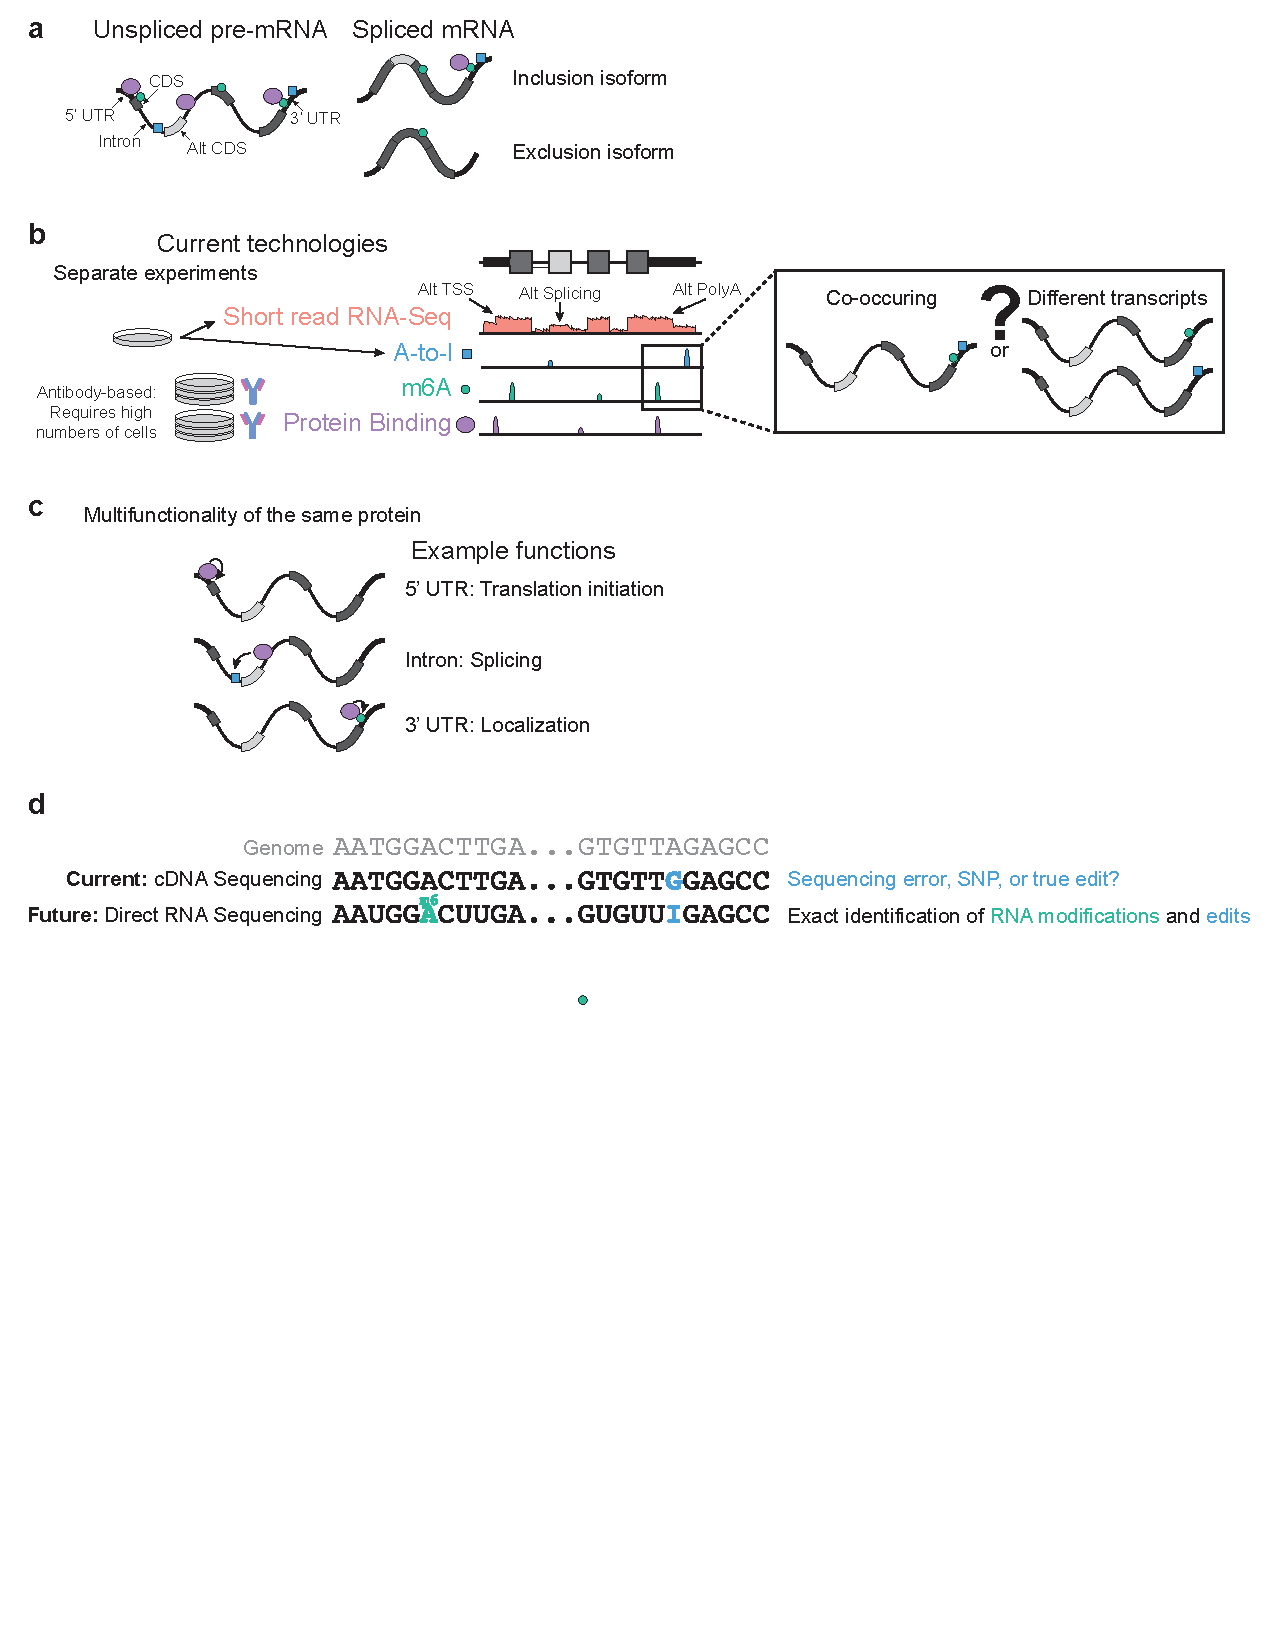
\includegraphics[width=5.8in]{figures/singlecell_future_methods}
  \caption[Unmet needs in RNA processing and potential future technologies.]{Unmet needs in RNA processing and potential future technologies.\\
\textbf{a.}~Left, example RNA transcript with RBPs (purple), A-to-I editing (blue), and m6A (green). Right,  possible inclusion and exclusion isoforms with different post-transcriptional modifications of splicing, m6A, RBP binding, and m6A modification.\\
\textbf{b.}~Current technologies allow for visualization of RNA abundance, A-to-I editing, m6A methylation, and protein binding, but cannot determine whether these occur on physically different or the same molecules.\\
\textbf{c.}~Technologies are needed to investigate multifunctionality of the same protein, e.g. if it performs different functions based on where it binds in the transcripts. Additionally, this would be interesting to study redundancy of different proteins such as splicing factors.\\
\textbf{d.}~Future direct RNA sequencing technologies would allow for direct identification of multiple RNA modifications and edits on the same transcript, unlike currently available technologies.}
\label{fig:singlecell_future_methods}
\end{figure}

\subsection{Across-cell distributions of RNA and protein with high-throughput technologies}

Beyond model organisms such as \emph{Caenorhabditis elegans}, the number of different cell types and niches in the body are unknown at the organism level \cite{Deppe1978-dd,Ellis1986-oz}. For example, in the neurodegenerative disease amyotrophic lateral sclerosis (ALS), protein aggregation in motor neurons of the spinal cord are thought to be the main cause of disease \cite{Da_Silva2014-dv,Polymenidou2011-ah}, but there are many other supporting cells in the spinal cord such as glia and astrocytes whose functions are are unknown. As a result, researchers either remove the entire spinal cord or laser-capture micro-dissect only the motor neurons from donors \cite{Aulas2012-uc,Gal2011-mg,Martinez2016-sv}. But the spinal cord is an integrated system of many cell types -- how do glia and astrocytes contribute to the progression of the disease? If instead researchers could perform single-cell capture of the entire spinal cord,  and then spatially reconstruct the cell types and locations without a priori knowledge \cite{Achim2015-sf,Mori2017-xr,Pettit2014-od,Satija2015-hi}, they then could focus on analyzing the differences in RNA and protein processing within and across, cell types and individuals, rather than making inferences based on incomplete information. Such a ``cell atlas'' would greatly inform the understanding of disease.

Indeed, a Human Cell Atlas (HCA) \cite{Linnarsson2016-dk,Regev2016-li,Wagner2016-mi} project is currently underway, where researchers are working towards establishing molecular and physical markers of cell types in the human body. In the future, it will be possible to ``align'' a transcriptome of interest to the HCA and obtain the closest cell types and cell locations, helping to provide a more complete understanding of human cellular biology. This will reducing the burden for researchers to painstakingly capture spatial locations of cells in the body when harvesting tissue, thus lowering the barrier for biological research and paving the way for discovery.


\subsubsection{Mutually exclusivity and co-occurrence of RNA features}

Future understanding of the interdependence of RNA features will require the measurement of multiple aspects of RNA processing at once. Current technologies to measure transcript abundance and over 120 possible nucleotide modifications \cite{Ferre-DAmare2003-to,Gilbert2016-pg,Li2014-dq,Saletore2012-fp,Sun2016-rk}, must be performed in separate, bulk experiments, and beyond correlations, the co-occurrence of these features on the same transcript is unknown (\Cref{fig:singlecell_future_methods}a). One potential method for measuring multiple features at once is direct sequencing of RNA and its modified bases, without creation of a cDNA template such as by the Oxford Nanopore MinION \cite{Goodwin2015-ca,Jain2016-yb,Loman2014-ss,Mikheyev2014-gd} or Pacific Biosciences Single Molecule Real-Time (SMRT) Sequencing \cite{Flusberg2010-yf}. These technologies can directly detect RNA modifications (\Cref{fig:singlecell_future_methods}b) such as m6A and inosine \cite{Carr2016-bc,Garalde2016-iw,Saletore2012-fp}, exon structure driven by alternative splicing in transcripts \cite{Karlsson2017-wy}, and help to answer the question, what percentage of cells have a modification or transcript structure? Unfortunately, these technologies are plagued with high error rates and this challenging problem of accuracy for single molecule sequencing will need to be addressed. Additionally, many of the library preparation methods for capturing entire transcripts measure only mature, poly-adenylated mRNA and not any byproducts of mRNA processing such as mirtrons or circular RNAs \cite{Salzman2013-ol}, which can be cell-type specific and for which other capture methods must be developed. Nonetheless, if the entire transcript is measured, these technologies would reveal the co-occurrence of relationships such as between alternative splicing and nucleotide modifications, shedding light on the co-dependence (or independence) of RNA processing elements.

Translation of mRNAs can vary from tissue to tissue, but has not yet been shown to vary from cell to cell. There are several methods for bulk samples to answer the question, which transcripts are actively translating? \cite{King2016-yp,Lesiak2016-ji}. BacTrap and RiboTag fluorescently label ribosomal subunits and then capture the ribosomal-bound transcripts to perform full-length transcript sequencing \cite{Lesiak2016-ji}. Ribosome profiling (also called ``ribo-seq'' or ``ribosome footprinting'') measures protected RNA fragments \cite{Brar2012-pj,Ingolia2009-zu,Ingolia2011-gf}, and can pinpoint the paused locations of ribosomes. All of these are possible to scale to the single-cell level but will have high rRNA contamination, and at the single-cell level, every nucleotide counts, so protocols must be optimized to be sensitive only to the molecules of interest.

Beyond coding sequences, there are many disease-associated mutations that occur in non-coding regions such as introns and 5'/3' UTRs, which are likely to influence its ability to form three-dimensional structures and can vary between cells. For example,  Thus, measuring RNA structure and binding partners at the single-cell level is a critical problem, but due to technical limitations, remains unsolved. Current methods for measuring RNA secondary structure, typically by selectively measuring only single- or double-stranded RNA, require high amounts of starting material, meaning, many thousands of cells as input \cite{Bevilacqua2016-gy,Flynn2016-am,Kubota2015-oj,Rouskin2014-uf,Spitale2013-aq,Wan2011-uw,Wan2014-sk}, thus averaging out the signal across many cells. Scaling these protocols down to single cells will be challenging, it will require tiny amounts of each reaction occurring in nanoliter volumes of captured cells. Double-stranded structure is also important in lncRNAs, as their functions range from inhibiting entire chromosomes (XIST) to sequestering RBPs (MALAT1) \cite{Engreitz:2016by}. Combining the measurement of RNA structure with RNA modifications will inform how individual nucleotides promote or inhibit certain RNA structures. Capturing the three-dimensional structure of RNA in single cells will be a challenging problem to solve, but will pay great dividends in understanding RNA biology.

Even if there existed the perfect high-throughput method of interrogating all possible nucleotide modifications, RNA structures, and translating transcripts, it is likely the subcellular context would be lost. Need to perform follow-up experiments showing the localization and dynamics of the different transcripts. These experiments would answer questions such as, what are the time-scales of RNA modifications and translational pausing? How transient are RNA structures and how do they affect localization of the mRNA? While High-throughput experiments can create millions of data points, they are merely a starting point, creating a scaffold upon which to build knowledge of RNA processing.


\subsubsection{RBP specialization in single cells}

While high-throughput transcriptomics from single cells is possible though imperfect, high-throughput proteomics in single cells is a challenging problem that remains to be solved. It is not yet possible to perform a massive ``sequencing-style'' experiment on proteins as their building blocks, amino acids, do not have Watson-Crick base-pairing rules. Instead, mass cytometry \cite{Chen2012-gb,Giesen2014-eb,Irish2006-qt,Spitzer2016-nt,Wu2012-dt} using antibodies conjugated to heavy metal isotopes has been applied primarily to immune and cancer genes, and could be applied to RBPs, specifically to ribosomes \cite{Wilson2012-zv}. Ribosomes have been shown to be specialized to certain tissues, and have been shown to require specific subunits for proper function \cite{Brombin2015-cw,Buszczak2014-yq,Shi2015-fh,Signer2014-zw,Gilbert2011-nr,Xue2012-fb}. Ribosomal dysfunction has been implicated in a wide variety of neurological disorders such as Alzheimer's disease and Charcot-Marie-Tooth disorder, as well as viral infections such as foot-and-mouth disease \cite{Ding2005-sr,Freed2010-dm}. Performing mass cytometry of ribosomal subunits could be used to investigate, what is the exact composition of ribosomal subunits of each ribosome in each cell (\Cref{fig:singlecell_future_methods}c)? Follow-up experiments showing how differently composed ribosomes function differently in binding preferences, translation rates, or localization would be needed. For true discovery, it is important to have the ability to shatter all proteins and reassemble them as in sequencing using technologies such as mass spectrometry \cite{Aebersold2003-yi,Wilhelm2014-tt}, but these have not yet been scaled to single cells and would require a dramatic reduction in cost to be accessible to researchers.

The concurrent measurement of RNA and protein would inform how RBPs specialize to different aspects of RNA processing in different contexts (\Cref{fig:singlecell_future_methods}d). An intermediate technology could be to measure RNA abundance and protein levels simultaneously. Seq-well, RNA-seq coupled with antibody-based markers has applied to immune genes \cite{Gierahn2017-ko}. Seq-well could be extended to RBPs, for example, to dissect families of related proteins, such as ribosomal subunits or splicing factors, relative to transcript abundance. However, a multiplexed approach measuring the sequence specificities of proteins in addition to the RNA abundance would be more informative.

For example, heart, brain and muscle all express members of the homologous RBFOX family at different levels \cite{Damianov2016-pa,Dredge2011-bk,Lovci2013-fr,Nutter2016-nu,Weyn-Vanhentenryck2014-vt}. RBFOX proteins have been implicated in splicing and in transcript stability \cite{Arya2014-po,Jangi2014-ww}, in some cases dependent on the localization of the protein \cite{Dredge2011-bk}. Understanding exactly which of RBFOX1/2/3 bind at different locations in the transcript would inform how these highly similar proteins have very specialized functions. There are existing methods for measuring RNA-protein interactions is cross linking and immunoprecipitation (CLIP)-Seq, which now has many variants (eCLIP/iCLIP/irCLIP) \cite{Haberman2017-at,Huppertz2014-jt,Van_Nostrand2016-qd,Zarnegar2016-zq} However, few RBP-RNA interaction sites exist relative to the total amount of RNA and due to the inefficiency of antibodies, these techniques require high numbers of cells as input to be able to detect even a few interaction sites. Scaling *CLIP-Seq to single cells will require substantial optimization of the protocol. Ideally, detecting several RBPs, their RBP-RNA interaction sites and the entire transcript could be measured, to provide insight into how homologous RBPs differentially bind in different cellular contexts and ultimately create a wide variety of distinct phenotypes. 

\subsection{Molecular organization in space and time}

How do different RNA isoforms influence the protein product? To capture the RNA-protein transformation, need technologies that combine RNA and protein measurements. For example, coupling of RNA-FISH with antibody-based immunofluorescence of the protein product would allow for visualization of differential isoform usage and protein localization. For example, if one isoform appears in cells where the protein is cytoplasmic while the other appears with a nuclear protein localization (\Cref{fig:singlecell_future_methods}e), this suggests that the different mRNA isoforms influence the localization signals of the protein. However, this only examines cells fixed in one state, and can only garner correlations but not causes -- need perturbations and/or dynamics to visualize how isoforms are differentially processed. For example, do the isoforms have different transcription or splicing kinetics? How do their differential sequence, modifications, editing, binding partners, and structure, contribute to localization and translation?

\subsubsection{Moonshot target: Live cell imaging of both dynamics and spatial organization of RNA processing}

Ideally, one could measure the phenotype of a cell, then perturb that same cell and observe the result. However, most single-cell technologies are destructive -- once you sample the cell, you can't put it back and see how it responds in a new situation. Live cell imaging of RNA and protein enables encoding information of both localization and time scales (reviewed by \citet{Buxbaum2015-eu}). However, imaging-based methods are low throughput as they cannot yet resolve individual molecules without significant signal amplification, or discover novel RNA molecules. Nonetheless, as smFISH began by measuring a single RNA and can now be multiplexed to visualize hundreds of molecules \cite{Shah2016-sn}, live cell imaging has started with a few RNAs at a time and will eventually expand to visualize poly-adenylation sites, editing, nucleotide modifications, RNA structure, and binding partners such as DNA, RNA, protein, and metabolites.

Just as transcription factors come together in pulses \cite{Cai2008-zl,Cohen-Saidon2009-ib,Hao2011-sp,Lahav2004-oq,Levine2013-nb,Lin2015-ax,Locke2011-tc,Nelson2004-tk,Purvis2013-fa,Yosef2011-jy}, RBPs that facilitate transcription and perform co-transcriptional tasks must also be aggregated in pulses, and are especially important for the assembly and disassembly of membrane-free organelles used in RNA storage and splicing such as paraspeckles, stress granules and the spliceosome. How does the cell ``know'' it is time to transcribe and ``tell'' the molecular components to convene in one place? How exactly do these molecules come together? Current methods for live cell imaging of transcripts are difficult because they require design of RNAs containing bulky hairpins, then adding the hairpin coat protein, creating large structure on the RNA molecule and possibly disrupting normal RNA processing \cite{Coulon2014-he,Hocine2013-if,Tyagi2009-jq}. 

Technologies to measure the assembly of these organelles in live cells will be necessary, labeling both RNA and protein with fluorophores. RNA could be labeled in cellulo fluorescently without adding much molecular weight \cite{Custer2016-gt}, with molecular beacons \cite{Santangelo2010-ry}, or with novel RNA-targeted CRISPR technologies \cite{Nelles2016-my}, provided the technique scaled to the single molecule level. The biggest challenges in optimizing the protocol to single molecules is signal amplification and multiplexing across multiple RNA molecules, but techniques from in situ sequencing could be applied to increase the number of fluorophores and increase the number of different transcripts measured. Given the ultimate system that images single RNA molecules in real time, would allow for real-time visualization of an RNA molecule's life.


\subsubsection{``Goldilocks'' balance: Single-cell multiomics}

Previously, it was thought that there are certain unalienable ``uncertainty principles'' in biology, such that one could not know both both the genotype and phenotype of a living cell \cite{Strippoli2005-ko} or both the cellular ``position'' (current cell state) and ``momentum'' (a cell's past or future, i.e. its lineage or differentiation trajectories) \cite{Shapiro2013-kk}. However, recent work in single-cell multiomics has turned these principles on their head [reviewed in \citet{Macaulay2017-tb}]. Both the genotype and phenotype can be measured from a single cell by capturing both DNA and RNA \cite{Macaulay2015-iz,Reuter2016-op}, and even coupling with measuring epigenomics and RNA \cite{Angermueller2016-rx,Hou2016-zi}. A cell's ``position'' and ``momentum'' can be inferred through algorithms that delineate cellular trajectories from phenotypic measurements such as RNA-seq, reviewed thoroughly by \citet{Cannoodt2016-mt}. While simultaneous capture of the (epi)genome and transcriptome have been major breakthroughs, there are many more aspects of cellular state that are still invisible to the sequencing eye. We expect more technologies to upend traditional thinking of what is possible at the single cell level.

The ability to simultaneously measure RNA and DNA has not yet been applied to questions of RNA processing, and there are many ``low-hanging fruit'' opportunities to study the question, are RNA features marked (epi)genomically in the DNA? With the simultaneous measurement of both the (epi)genetic context and transcriptome, researchers can observe mutual exclusivity/co-occurrence of DNA features and RNA processing, as with within RNA features (\Cref{fig:singlecell_future_methods}a). For example, there is evidence that alternative splicing regulation is influenced by polymerase speed, GC content and epigenetic marks \cite{Fiszbein2017-vl,Kornblihtt2013-gm,Tilgner2010-ia}. These simultaneous measurements would help to to answer the questions, how do chromatin modifications \cite{Calo2013-xx,Ng1999-tp}, four-dimensional genome structure \cite{Dekker2017-yg}, and single nucleotide polymorphisms influence alternative splicing? In a perfect world, to study the interplay between DNA and alternative splicing, one could observe genomic features, transcription speed, and alternative splicing simultaneously, for all transcripts. Alternative splicing is but one facet of RNA processing, and these multiomics measurements would help to answer, Is an RNA's fate encoded in the (epi)genome?

Another method to create additional context for each individual cell is to combine high-throughput measurements with genome editing such as with CRISPR/Cas9, allowing for dissection of complex phenotypes in mammalian cells at large scales. For example, Perturb-seq is a method that combines knockdown of genes using CRISRPi with single-cell RNA-seq, and was used to study the unfolded protein response \cite{Adamson2016-nu} and effect of lipopolysaccharides on dendritic cells \cite{Dixit2016-sa}. This created a computational scientist's dream dataset, as for each gene that was knocked down, there was a control dataset, and thus for developing algorithms, one could always have a negative control to check with. Perturb-Seq could be applied to study any aspect of RNA processing, e.g. systematically knocking down ribosomal subunits or splicing factors, enabling fine-tuned dissection of high-level regulatory units.

So far, the technologies we have discussed have focused on observing a cell's present, but recent developments have enabled encoding of a cell's history or lineage in its genome using CRISPR/Cas9 \cite{Frieda2017-vv,McKenna2016-yi}. Coupling phenotypic measurements such as RNA-Seq or smFISH with lineage tracing, would allow for comparison of present cell state while considering cellular time. Using phylogenetic techniques, cell lineages could be reconstructed and even the times at which cells asymmetrically divided to change fates could be found. If RNA-seq encodes a cell's present, then its traced lineage encodes its past. This lineage tracing method, coupled with direct RNA sequencing, would help to understand how developmentally regulated RNA processing events such as RNA editing, m6A, and alternative splicing, are finely tuned in different lineages. Do all cells that were committed to a particular lineage also have certain RNA processing events? This could indicate inheritability of the event, either encoded through the genome or by asymmetrically dividing the RNA content of a mother cell. The simultaneous measurement of a cell's past and present will illuminate a deeper understanding of cellular processing and will enable the computational prediction of cellular futures.

\section{Conclusions}

Each RNA molecule lives a rich, fulfilled life, and while advances single-cell technologies have greatly expanded our understanding of RNA processing, many questions remain. How do the many transient aspects of RNA, such as nucleotide modifications, binding partners, 3D structure, and localization, affect each other? What is the effect of non-RNA, such as DNA, protein, or metabolites, on RNA? Where in the cell does an RNA molecule travel? What does it interact with on the way? Finally, when a feature is variable, is it noise or is it functional? Maybe the noise itself is functional \cite{Arbel-Goren2014-iq,Dueck2016-mr,Symmons2016-xn}? In conclusion, there are ample opportunities for application of current and future technologies to understanding the entirety of an RNA's existence, and ultimately the molecular processes that drive diversity in cell types across human life.

\section{Acknowledgements}
Chapter 1, in full, is currently being prepared for submission for publication of the material. Botvinnik, Olga; Song, Yan; Yeo, Gene W. The dissertation author was the primary investigator and author of this material. 